Given an addition of auto-scaling, it is now necessary to progress to
evaluation. This section contains a more thorough definition of what entails
successful modification of current Kubernetes auto-scaling behavior, the metrics
used to determine if efforts were successful, an analysis of the control groups
with which the new predictive auto-scaling will be compared, a description of
the environment and process used for evaluation, the results of said
evaluations, and the real world impacts of this thesis' findings.

\section{Goals of Evaluation}

In the introduction section of this thesis, we defined success as implementing
modifications to Kubernetes that will increase the summation of the
efficient resource utilization and quality of service metrics. Careful
evaluation will confirm whether we succeeded in this objective. In all, we will
seek to determine both the extent and significance of the addition of predictive
auto-scaling in comparison to other methods of allocations resources with
respect to our goal summation, and highlight the scenarios in which the addition
of predictive auto-scaling is the most, and the least, beneficial.

\subsection{Predictive Auto-scaling's Impact}

One important aspect of evaluation will be presenting a number of different
scenarios, based on independent variables that will be discussed later, in which
to evaluate predictive auto-scaling in comparison to the alternative methods
of assigning resources. This type of evaluation will focus on how predictive
auto-scaling is an improvement, or regression, on the currently existing
options. Furthermore, this type of evaluation will focus on to what extent
predictive auto-scaling's difference from current implementations,
is statistically and practically significant. Finally, this type of evaluation will
provide a number of visualizations and summary statistics, allowing for
easily accessible comparisons between different types of resource assignment
in different scenarios.


\subsection{Scenario Analysis}

Our evaluation will also attempt to provide
further insight into predictive auto-scaling
through analyzing the impacts of predictive auto-scaling in different scenarios.
In other words, we will seek to identify the scenarios in which benefits or
detriments of predictive auto-scaling are the most pronounced, and also the
scenarios in which predictive auto-scaling has little impact. This method of
analysis will be useful in recommending when to enable predictive auto-scaling
and also will likely suggest avenues for future work.



\section{Evaluation Metrics}

Before progressing any further, it is important to state the metrics we will use
to measure the efficacy of predictive auto-scaling. We seek specific metrics relating to
the general concepts of efficient resource utilization and quality of service.
A selection of a ``typical'' service to run on Kubernetes influences how exactly
we will measure efficient resource utilization and quality of service. We posit
a web service as the best choice for a representative application. A number
of factors support our decision. First, Kubernetes is built for running
long-term, stable service jobs, and a well-built web application desires to be
both long-running and crash free \cite{k8s-design-overview}. Second, Kubernetes
focuses on running ephemeral, containerized applications which can be started or
stopped at any time. Containerized web services achieve these goals as, as
long as the database layer is abstracted, web applications are stateless and can
restart with few ramifications. Third, applications on Kubernetes should be
concurrent, meaning replicas can be added or removed to divide the work any
individual application must handle. Stateless web services are easily
parallelized, as the requests can be easily distributed across all of the
replicas. Finally, much of the appeal of the simplicity of Kubernetes is that a
user can construct a containerized application and then pass it to an
externally managed Kubernetes cluster for hosting. This hosting simplicity is
particularly appreciated by burgeoning startups, who typically develop web
applications and may face extreme variance in external demand.

\subsection{Efficient Resource Utilization}

We define efficient resource utilization as a measure of whether an application
has enough, but not too many resources given to it by the operating system or
the cluster manager. For example, editing a text file in Vim on a supercomputer
would be terrible efficient resource utilization since editing a text file
requires only a small fraction of the supercomputer's available CPU and memory,
meaning the unneeded resources are wasted. In contrast, running a web browser on
a laptop is proper efficient resource utilization, because a web browser requires
an appropriate percentage of the laptop's available resources.
In the context of Kubernetes, an application with
poor efficient resource utilization would be a web server
that uses many replica pods, each reserving considerable resources,
to serve a very low volume of web requests. In such a situation, the resources
reserved for the application would be entirely underutilized.

Specifically, we measure efficient resource utilization with respect to
Kubernetes through examining the percentage of idle CPU.
The amount of CPU that a pod reserves is the summation of
all resources that containers within the pod reserve
\cite{k8s-compute-resources}. If our application is only using a small amount of
that reserved CPU to run, than a large amount of CPU will be left idle. The
larger the percentage of CPU that is left idle, the worse the efficient resource
utilization, as many resources are just sitting unused.
We measure our specific metric for efficient resource
utilization in percentage of CPU that is idle and we name it
\code{IdleCPU}. When we use this metric to indicate efficient resource utilization,
if the ERU value is high, the application is not using resources efficiently. If
the metric is low, the application is using resources efficiently.\footnote{In a
similar vein, a low measure for quality of service is actually preferable to a
high value for quality of service when we are measuring quality of service
through request response time. However, when summing ERU and QoS we consider
the inversion of this measurement of ERU, meaning a large summation of ERU and
QoS is preferable to a small summation of ERU and QoS.}

Our decision to use idle load to measure efficient resource utilization
in Kubernetes makes the assumption that
creating pods equates to reserving the pod's resources such
that they cannot be used by other pods.
In the default case, the previous statement is not necessarily true,
yet it is possible to craft specialized pods which validate this equality. To
start, remember that pods contain containers. When Kubernetes receives a pod, it
seeks to schedule all of its containers on a physical node within the cluster.
By default, containers within the pod run with no bounds on their CPU and memory
beyond the constrictions of the physical node on which they are scheduled. As such,
declaring $x$ number of pods does not give any guarantees of resource usage, as
the amount of resources available to the containers within the pod vary
drastically based on their specific node \cite{k8s-limit-range}. Without
modification, this variability would undermine \code{IdleCPU} as our metric for
ERU.

Fortunately, there is a way to configure Kubernetes such that a pod
equates to a static number of resources.\footnote{Right now in Kubernetes,
resources relates to either CPU or memory. CPU is requested in cores. Memory is
requested in bytes of RAM.} This configuration involves
setting resource requests and limits for each container within the pod. A
resource request for a container indicates the minimum amount of resources that
should always be available. A pod will not be scheduled on a node within the
cluster, unless that node can guarantee the requested amount of resources to all
containers within the pod. A resource limit for a container indicates the
maximum amount of resources that a container can claim. Depending on the
resource, a container exceeding the maximum amount of resources will either be
throttled (CPU) or killed (memory).\footnote{It is also possible to configure
Kubernetes such that a container using too much CPU is killed.} A pod's resource
request/limit is the summation of the resource request/limit for all of its
containers. Setting a container's, or pod's, resource request equal to its
resource limit essentially guarantees that the existence of a pod represents the
claiming and utilization of a static amount of resources
\cite{k8s-compute-resources}. Ensuring static provisioning
is reserving a consistent amount of resources
allows us to still examine idle CPU percentage, our way of investigating
efficient resource utilization.

The efficient resource utilization metric has direct links to the costs of
running applications on a cluster manager. If applications are given resources
they do not need, and the cluster manager does not reclaim these unused
resources, then additional applications added to the cluster must claim new
resources. The inability to utilize inefficient applications' wasted resources
requires the expansion of the cluster. This increase in cost will be felt
both by those running the cluster and those running an application on the
cluster.


\subsection{Quality of Service}

We additionally define quality of service as a measure of how well an application
is accomplishing its goal. There does not exist a singular consistent specific
metric for measuring quality of service, as measures of quality of service are dependent on
the specific application. Furthermore, it is difficult to measure quality of
service as a variety of difficult-to-control-for external factors impact an
application's ability to perform its goal.

In the context of the typical web application run on Kubernetes, we measure
quality of service based on the server side
\textit{response time} to an HTTP request. An application
with a high quality of service will have a low response time, while an
application with a low quality of service will have a high response time. Our
specific metric for quality of service will be measured in seconds.

The quality of service metric has links to the type of application which can be
run on Kubernetes. As Kubernetes supports as best as possible a high quality of
service, more and more important applications will run on Kubernetes. For
example, if Kubernetes works to improve the quality of service of an
application, important web applications serving vital medical data or political
information will seek Kubernetes as a platform on which to run.


\subsection{Summation of ERU and QoS}

We are most interested in testing for an improvement in the summation of
efficient resource utilization and quality of service metrics. It is
easy to improve quality of service by decreasing efficient resource
utilization, as we can just assign the application the largest amount of
resources it could ever need. It is equally easy to improve efficient resource
utilization by decreasing quality of service, as we can just assign an
application the fewest amount of resources it will ever use. As such, we want to
ensure that this thesis improves efficient resource utilization or quality of
service, without negatively impacting the other. This realization leads us to
evaluating our modifications to auto-scaling by measuring its impact on the
summation of efficient resource utilization and quality of service.

While conceptually summing efficient resource utilization and quality of service
is simple, care must be taken when combining the specific metrics of
\code{IdleCPU} and \code{ResponseTime}. The metrics are measured in unrelated
units. Furthermore, the scale for these metrics may be entirely different,
meaning that small changes in one could completely overshadow larger changes in
the other. Additionally, for both \code{IdleCPU} and \code{ResponseTime} low
measures are desirable, while intuitively with summation of ERU and QoS, high
measures are desirable.

We combine these ERU and QoS measurements through the following process.
First, we gather all measurements of ERU and QoS,
distinguished by the variables $E_{A}$ and $Q_{A}$ respectively, from our
predictive and reactive measurements for a single combination of independent
variables. Next, we define $e_{t}$ and $q_{t}$ as the
respective ERU and QoS measurements at time $t$. We first
normalize these measurements through calculating their respective z-scores,
by first subtracting the individual observation value
from the mean of all observations, and then dividing by the standard deviation of all
observations. This operation leaves us with $ne_{t}$ and $nq_{t}$ respectively.
Our next step relates to how we interpret measurements for ERU and QoS, and how
we interpret measurements for the summation of ERU and QoS. With the current
metrics we use for measuring ERU and QoS individually, smaller values indicate
``better'' performance. However, with the summation of ERU and QoS, it makes
intuitive sense that higher values should indicate ``better'' performance.
Thus, we negate $ne_{t}$ and $nq_{t}$, before we finally sum
$-ne_{t}$ and $-nq_{t}$ together to get $s_{t}$, where $s_{t}$ is the summation
of ERU and QoS at time $t$.
In short, we add the negation of the z-score for
ERU and QoS. Mathematically, this process can be written as
follows:

\begin{align*}
  ne_{t} &= ((e_{t} - \mbox{MEAN}(E_{A})) / \mbox{STDDEV}(E_{A})) \\
  nq_{t} &= ((q_{t} - \mbox{MEAN}(Q_{A})) / \mbox{STDDEV}(Q_{A})) \\
  s_{t} &= -ne_{t} + -nq_{t}
\end{align*}

Given a measurement of the summation of ERU and QoS for a set
of observations, in which ERU and QoS have an equal impact in
the summation, it is now possible to compare the summations of ERU and
QoS within the different scaling methods or traffic patterns included
in our evaluation trials.



\section{Control Groups}

\subsection{Static}

The first, and the simplest method, of scaling pods is \textit{static}
provisioning. Static provisioning requires one wishing to deploy an application on
Kubernetes to determine ahead of time a constant amount of pods for that
application. Any desire to update that static value will require a manual
change. Put simply, with the static method there will be a constant number of
pods, and the application will have a constant amount of resources, throughout
its entire lifetime, regardless of the amount of work the application is asked
to perform.

There are multiple possible heuristics for statically assigning resources to an
applications, as it is possible to over, under, or average provision.

\begin{itemize}
  \item \textbf{Over Provision}: With over provisioning, an application is given
    the greatest amount of resources that it will ever require. With respect to
    horizontal pod auto-scaling, over provisioning means the user of the
    application statically sets the replication controller to ensure that $x$ pods
    always exist, where $x$ is the number of pods needed to
    maintain high quality of service when the application is
    asked to perform the most work.\footnote{In this discussion, references to
    \textit{most}, \textit{least}, and \textit{average} work assume that there
    exist bounds on the work the external environment can ask the application to
    do.} While over provisioning ensures a high quality of service, it has extremely
    poor efficient resource utilization.

  \item \textbf{Under Provision}: With under provisioning, an application is
    given the least amount of resources that it will ever require. Again, in the
    context of horizontal pod auto-scaling, under provisioning leads to user to
    statically set the replication controller to ensure the existence of
    $y$ pods, where $y$ is the number of pods needed to maintain quality of
    service when the application is asked to perform the least work. Under
    provisioning ensures efficient resource utilization, as the application will
    never reserve any resources and then leave them idle. However, in all
    situations except for when the application performs the minimum possible
    amount of work, quality of service will suffer because the application does
    not have enough resources.

  \item \textbf{Average Provision}: With average provisioning, an application is
    given the average amount of resources that it needs. With respect to
    horizontal pod auto-scaling, average provisioning guides the user to
    statically set the replication controller to maintain $z$ pods, where
    $z$ is the number of pods needed to maintain quality of service when the
    application is asked to perform the average amount of work. Average
    provisioning can be seen as somewhat of a middle ground between under and
    over provisioning, offering decent quality of service and efficient resource
    utilization.
\end{itemize}

Ultimately, we do not devote significant time to
considering any type of static provisioning, as we are confident that it will at
best be equal to reactive auto-scaling. Thus if our implementation of predictive
auto-scaling outperforms reactive auto-scaling, we are confident that it will
also outperform any type of static provisioning, and as such we only compare
predictive auto-scaling to reactive auto-scaling in our evaluation.


\subsection{Reactive Auto-scaling}

Additionally, previous to this thesis, it was possible to scale applications in
Kubernetes using horizontal, reactive pod based auto-scaling. We examine the implementation
and utilization of this method of scaling in depth in the \textit{Autoscaling in
Kubernetes} section, so we will not repeat it here.

However, some additional detail assists in understanding the potential values of
CPU utilization percentage that result from reactive horizontal auto-scaling.
Remember that the current implementation of reactive horizontal auto-scaling
occurs by having the auto-scaler create sufficient replica pods such that each
replica pods operates within a specified range of CPU utilization percentage.
\footnote{If we decide to enact resource requests\/limits on our replica pods, we can also
calculate the exact amount of resources being utilized, as opposed to just a
percentage. However, we are not particularly concerned about non-percentage
values because we measure efficient resource utilization using CPU utilization
percentage, instead of total CPU utilization.} If all replica pods initialize
and share in the work immediately, than we could expect CPU utilization
percentage to consistently stay within a small range of the value the user
specified. For example, if the user instructed the auto-scaler to auto-scale
such that all pods utilized 70\% of available CPU, and the range was $\pm 2$,
then we would expect CPU utilization, and thus efficient resource utilization,
to stay within $68 - 72$ CPU utilization percentage.
However, our justification for introducing prediction
the horizontal pod auto-scaling is an understanding that replica pods will not
always immediately initialize. In the times in which we are waiting for our pods
to initialize, we can expect CPU utilization to derivate from the expected
range. Establishing reactive horizontal pod auto-scaling as a contrl group
assists us in determining whether the addition of prediction improves upon what
existed in Kubernetes before this thesis began.



\section{Independent Variables}

We examine two independent variables, traffic request pattern and pod
initialization time, with respect to the different scaling types' performance.
In other words, for under-, average-, and over-static, reactive, and predictive
auto-scaling, we examine the impacts of varying the request pattern of traffic
to our testing application and the impacts of differing pod initialization
times. This allows us to determine under what combinations of traffic request
patterns and pod initialization time predictive auto-scaling is most effective,
and also under what combinations it is the least effective. Furthermore, because
we utilize the same independent variables for all of the different scaling
types, and because these independent variables are relevant to all scaling
types, we can make comparisons across the scaling types. For example, we could
determine that predictive auto-scaling outperforms reactive auto-scaling most
when pod initialization time is lengthy and the traffic pattern is a simple
linear slope, but predictive auto-scaling exhibits very little difference from
reactive auto-scaling when pod initialization time is very small and we see a
\textit{flash crowd} traffic pattern.

\subsection{Pod Initialization Time}

As will be discussed in detail in the later \textit{Tools} section, we've created a web
server application that allows us to specify any \textit{pod
initialization time} we desire. As such, we have considerable flexibility with
respect to what initialization time values we test. To begin, we decided to test the
following values: 5s and 135s.

We believe 5s and 135s are important independent variables to test because they
are indicative of different classes of applications that could be run on
Kubernetes. A pod initialization time of 5s is commonly found among web
application frameworks, as we showed when writing a simple HTTP server in Go and
using the Spring Java web application framework \cite{spring}. There web
frameworks initialized, and were ready to serve requests, in 1s and 5s
respectively. It is our strong belief that any web framework that simply
needs to initialize, without any external communicating our data, will
accomplish this task in under 5s. Thus, testing a pod initialization time of 5s
allows us to consider how any web application framework would perform with
predictive auto-scaling.

We derive a pod initialization time of 135s from a simulation of downloading a
shard database file, loading it into a database, and then starting a web
application to process data from said database. More specifically, our sample
pod downloaded a 25.2MB file and then batch inserted it into an Elasticsearch
database \cite{elasticsearch}. It then started a web application framework. In
all, this process took approximately 135s, although it is easy to imagine the
time varying based on the size of the initial shard file. The file we downloaded
came from an ElasticSearch tutorial on prepopulating a database
\cite{elasticsearch-import-some-data}, and thus we believe it is a fairly
representative size. By examining pod initialization times of 5s and 135s, we
are confident that we are capturing the majority of the potential use cases for
predictive auto-scaling.

We believe that there will be a \textit{sweet spot} of pod initialization times
for which predictive auto-scaling demonstrates the most benefits over reactive
auto-scaling. Obviously the smaller the pod intialization time value, the lesser
the difference between reactive and predictive auto-scaling, as predictive
auto-scaling predicts into the future a time closer and closer to the current
moment. However, the larger the pod initialization time value, the further into
the future we must predict the state of the application. While large pod
initialization times have the potential for considerable benefits when using
predictive auto-scaling, we can only realize that potential if predictions of
future application state are accurate. As the prediction window gets larger and
larger, accuracy becomes substantially more difficult to obtain.


\subsection{Traffic Request Pattern}

We are also interested in the impacts of different traffic patterns on scaling
performance. As such, we send our test web server application web requests in a
variety of patterns and examine which traffic pattern the scaling method handles
well, and which traffic pattern the scaling method does not handle well.
Moreover, we also examine scaling methods in relation to each other with respect
to different traffic patterns, seeking to answer for which traffic patterns
predictive auto-scaling is beneficial and which traffic patterns predictive
auto-scaling is detrimental or meaningless.

In this thesis we examine four different traffic patterns that we feel are
fairly indicative of the different traffic patterns a web application may face.
We entitle these patterns \textit{step-ladder}, \textit{jagged-edge},
\textit{increase-decrease}, and
\textit{flash-crowd}.\footnote{There are of course an infinite number of traffic
patterns that we could examine, and examining other options is an exciting
opportunity for future work.} We describe each of these patterns, and offer a
visual representation for each, below. Each pattern runs for at least twenty
minutes and at most forty minutes, and makes at most 20 requests per second.\footnote{All
traffic patterns have a start and end buffer at which they receive
only 1 request per second, to ensure we do not immediately overload the
application.} These values were chosen to give
space for the lengthier pod initialization times and to keep the network from
becoming too congested respectively. We can imagine the all traffic seen by a
typical web server as being composed of different combinations of these patterns
across longer time spans.

\begin{itemize}
  \item \textbf{step-ladder}: The traffic pattern \textit{step-ladder}, visible
    in Figure \ref{fig:step-ladder}, represents a web server which faces a load
    pattern which increases immediately at predicted intervals. This scenario
    can be seen as representing, for example, an video streaming website which
    experiences predictible increases in traffic as different shows are
    streamed. This traffic pattern begins with 1 request per second for 3
    minutes, before immediately increasing to 4 requests per second. The process
    of increasing by 3 requests per second and then staying constant for 3
    minutes continues for 6 more iterations until it reaches 19 requests per
    second.

    \begin{figure}[!h]
      \centerline{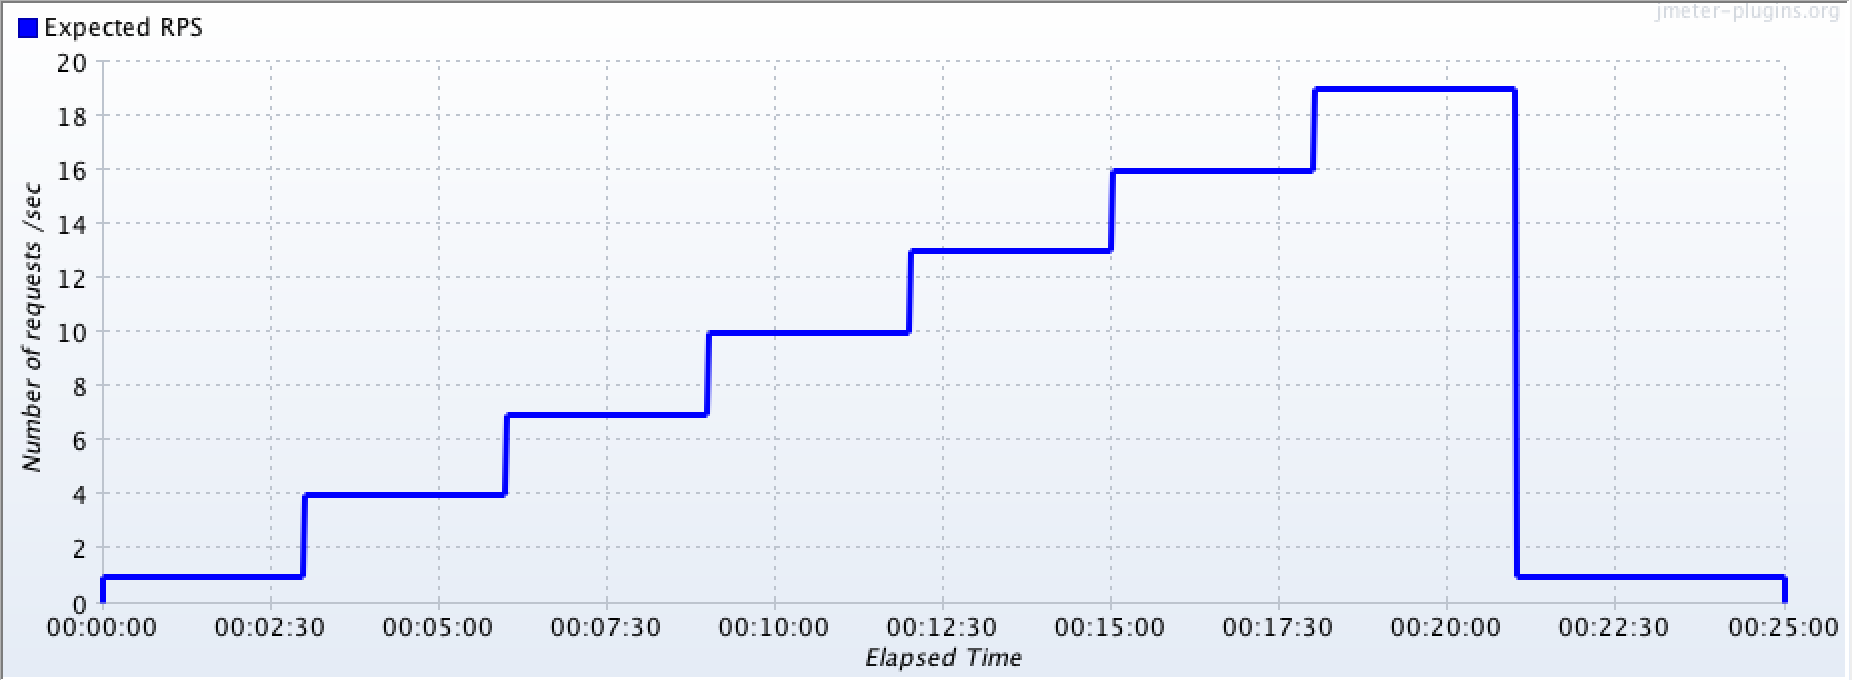
\includegraphics[scale=.4]{step-ladder.jpg}}
      \caption{The step-ladder Traffic Pattern}
      \label{fig:step-ladder}
    \end{figure}

  \item \textbf{jagged-edge}: The traffic pattern \textit{jagged-edge}, visible
    in Figure \ref{fig:jagged-edge}, is similar to \textit{step-ladder},
    although it reflects a more gradual increase and decrease in load. Thus, it
    applies to a similar scenario as \textit{step-ladder}. It begins at 1
    request per second before 3 minutes before increasing to 10 requests per
    minute over the course of 5 minutes. It then decreases to 5 requests per
    second over the course of 2 minutes. This pattern of increasing by 10
    requests per second over the course of 5 minutes and then decreasing by 5
    requests per second over the course of 2 minutes continues until reaching 20
    requests per second, and which point we transition to the end buffer period
    of 1 request per second for 5 minutes.

    \begin{figure}[!h]
      \centerline{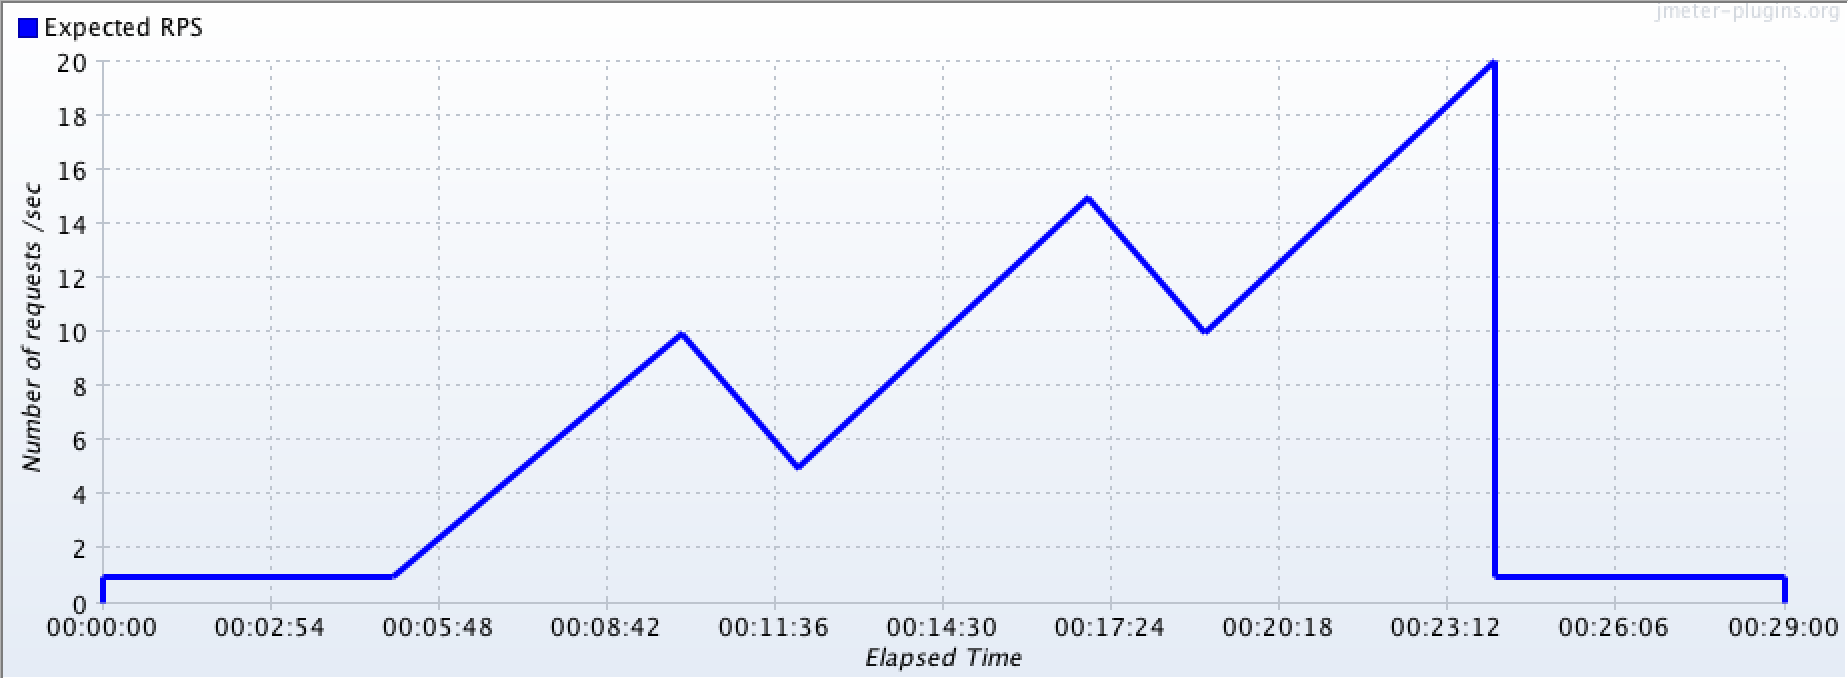
\includegraphics[scale=.4]{jagged-edge.jpg}}
      \caption{The jagged-edge Traffic Pattern}
      \label{fig:jagged-edge}
    \end{figure}

  \item \textbf{increase-decrease}: The traffic pattern
    \textit{increase-decrease}, visible in Figure \ref{fig:increase-decrease},
    represents a web server facing constantly increasing and then constantly
    decreasing load. This scenario can be seen as representing, for example, a
    restaurant in which people increasingly visit the site as it becomes closer
    and closer to a meal time, and decreasingly visit the site as a meal time
    becomes farther and farther away. After five minutes of initialization at
    1 request per second, our load
    generator builds from sending 1 request per second to 20 requests per
    second over the course of 15 minutes. After reaching the apex, the traffic
    generator then reduces from sending 30 requests per seconds to sending 1
    request per second, again over the course of 15 minutes.

    \begin{figure}[!h]
      \centerline{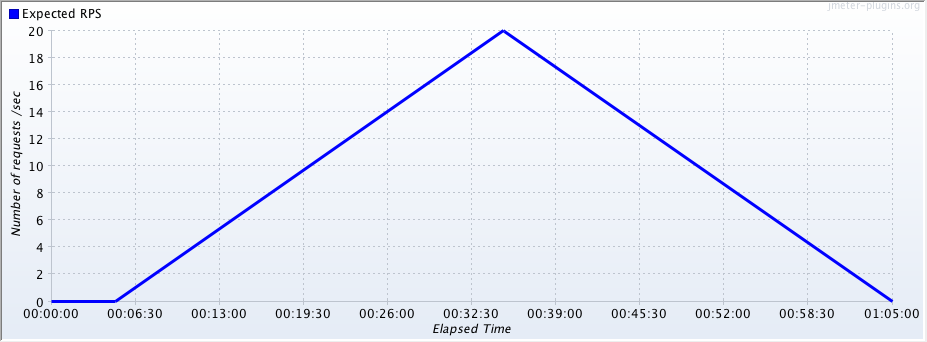
\includegraphics[scale=.4]{increase-decrease.jpg}}
      \caption{The increase-decrease Traffic Pattern}
      \label{fig:increase-decrease}
    \end{figure}

  \item \textbf{flash-crowd}: The traffic pattern \textit{flash-crowd}, visible
    in Figure \ref{fig:flash-crowd}, represents a web server facing a suddenly
    increasing, and then suddenly decreasing, amount of load. This scenario is
    indicative of, for example, a news website which will suddenly receive a
    short-lived burst of traffic when a major story hits. After five minutes of
    sending 1 request per second, our load generator
    builds from sending 1 request per second
    to sending 5 requests per second, over the course of 5 minutes. Then, in
    just 2 minutes, our load generator jumps from sending 5 requests per second
    to sending 20 requests per second. After reaching the apex, the traffic
    generator decreases from sending 20 requests per second to sending 5
    requests per second, again in just 2 minutes. Finally, our load generator
    decreases from sending 5 requests per second to 1 request per second, over
    the course of 5 minutes, before transitioning to the end buffer period of 1
    request per second for 5 minutes.

    %% We use flash-crowd-short although we refer to it as flash-crowd.
    \begin{figure}[!h]
      \centerline{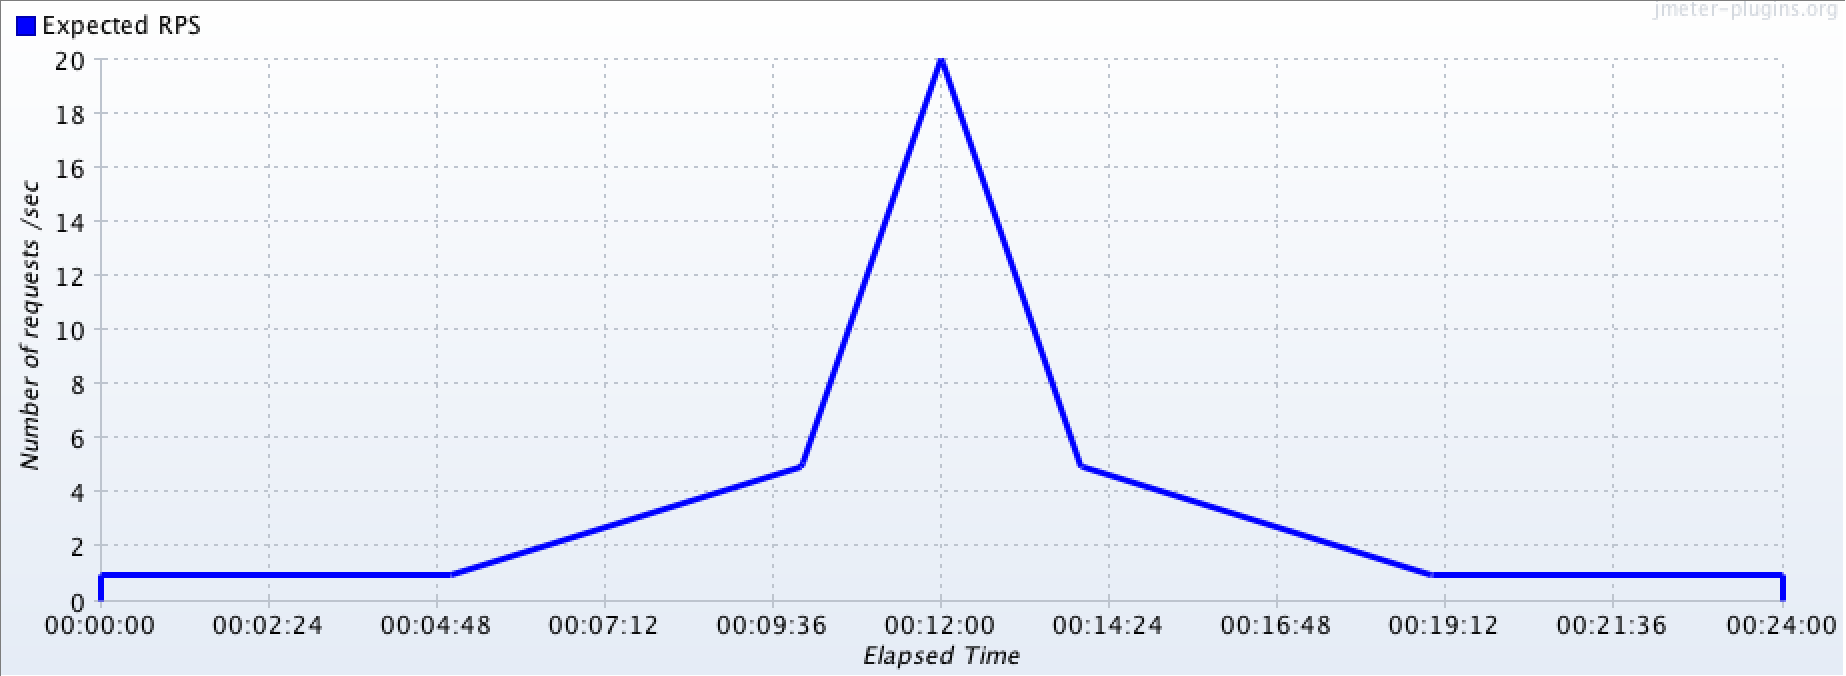
\includegraphics[scale=.4]{flash-crowd-short.jpg}}
      \caption{The flash-crowd Traffic Pattern}
      \label{fig:flash-crowd}
    \end{figure}

\end{itemize}



\section{Methodology}

Kubernetes does not currently contain either the tools or processes for
performing the evaluation this thesis needs.
This section gives an overview of tools and processes
we created for testing different types of scaling in Kubernetes.

\subsection{Tools}

Pursuing the evaluation method previously outlined in this thesis requires both
the creation of new tools and the utilization of previously existing open-source
tools.

\subsubsection{test-server}

We seek to measure variations in a web server application's
efficient resource utilization and quality of service across a variety of
scaling methods. Many of the previous sections of this thesis, and the majority
of this thesis' contributions to Kubernetes, relate to implementing predictive
horizontal auto-scaling as a new scaling method. Yet, to evaluate we must also
create a web server application. Ultimately, the created web server application,
entitled \textit{test-server}, allows us refined control over the independent
variables we wish to control during experimentation. \textit{test-server}
is a HTTP server written in Go. It defines two API
endpoints, ``/" and ``/ready".

\begin{itemize}
  \item \textbf{``/" - Load}: Traffic generators simulating user requests
    sends GET requests to the endpoint at ``/", also known as the \textit{Load} endpoint.
    This endpoint has two functions. First, it must perform a task that is
    somewhat CPU intensive so that our application uses enough CPU that
    auto-scaling may be triggered. Second, it must record the percent of idle CPU
    and an estimation of request response time as well as measures of
    efficient resource utilization and quality of service respectively. The
    function assigned to handle the GET request accomplishes these tasks as
    follows. Upon receiving a GET request to this endpoint, the handler function
    records the start time of the function. It then executes a computationally intensive
    task, which we define as repeatedly encrypting a password. Once this task
    is over, we once again record the time and check the idle CPU percentage
    through parsing the output of the \textit{top} Unix command.
    Having these two values allows us to calculate average amount of idle CPU
    and function execution time, which function as measurements of
    efficient resource utilization and quality of service. The function then
    records these values as a new point in the database, along with
    an indicator of the values of independent variables in place for this trial
    (i.e. pod initialization time, scaling method, traffic pattern). The function finishes by
    returning a status code of 200.
  \item \textbf{``/ready" - Ready}: The \textit{Ready} endpoint is used to allow
    us fine grained control over pod initialization time during experimentation.
    Kubernetes determines if a pod is initialized based on a
    \textit{ReadinessProbe}. This probe was discussed in greater detail earlier,
    but suffice to say it works by defining an HTTP endpoint that returns a
    successful status code if the pod is initialized. During experimentation, we
    are particularly interested in how different pod initialization times impact
    predictive auto-scaling. Thus, we utilize the following setup.
    First, when defining our pod, we specify the \textit{ReadinessProbe} should
    use ``/ready" as the HTTP endpoint. The function handling responses for
    requests to ``/ready" works by reading in an environment variable indicating
    the pod initialization time value we wish to test.\footnote{Any method of
    running containers, whether locally during testing or in a pod on
    Kubernetes, allows us to easily set environment variables.} The function parses this
    time, and waits that amount of time before returning a status code of 200.
    This wait ensures that we can control exactly when the
    \textit{ReadinessProbe} receives a successful response, and thus can
    control exactly the amount of time before a pod initializes.
\end{itemize}

This application closely fits within the guidelines microservice theory
establishes and it is easy to containerize it and then run it on Kubernetes. It
is \textit{focused}, as it performs the single task of responding to HTTP
requests. It is \textit{stateless}, as all containers communicate with an
external database, that is not stored within the container. The container can be
deleted and restarted at anytime with no errors or sustained interrupts.
Finally, the container can easily be replicated and run concurrently, as
a load balancer can distribute discrete requests across multiple replica HTTP
servers with no threat of race conditions. It is thus simple to package this
web server into a container, and then package said container into a pod.

As was previously mentioned, the pod containing the container for this
application implements a \textit{ReadinessProbe} pointing to the ``/ready"
endpoint. Additionally, the pod limits and requests an explicit amount of CPU,
currently .1 cores, for the container running the application. This ensures
measures of efficient resource utilization are consistent across scaling methods.
Finally, our pod contains a number of environment variables including
\textit{SCALING\_METHOD} and \textit{INITIALIZATION\_TIME} which allow us the
fine grained control previously mentioned. Additionally,
regardless of the scaling method, we define a replication controller for
ensuring whatever the scaled amount of pods exist, and a service for balancing
requests across all \textit{test-server} containers and exposing
\textit{test-server} to an external IP address that can receive our generated
traffic.


\subsubsection{InfluxDb}

Our evaluation strategy generates an immense amount of time-series data, which
we need to store in a database that we can later query and manipulate.
\textit{InfluxDB}, an open-source time-series database from InfluxData, is a
natural choice for recording such data. InfluxDB makes it easy to collect,
store, manage, and visualize the large amount of data that we generate.
InfluxDB provides a simple HTTP API which we use both for recording our data
throughout are evaluations, and also for querying and modifying later.
Finally, InfluxDB has a variety of hosting options, meaning our containerized application
does not have to hold any data, and thus remains stateless and concurrent.


\subsubsection{JMeter}

As mentioned in the discussion of independent variables, we need to generate
substantial traffic conforming to a specific pattern. Fortunately there a
variety of open-source tools that can assist us in this task. Ultimately,
we selected Apache JMeter \cite{apache-jmeter}. JMeter has
considerable functionality, but most appealing is its \textit{Throughput Shaping
Timer} plugin \cite{throughput-shaping-timer-plugin}. This plugin allows us to
use JMeter to send HTTP requests with a very specific pattern, by specifying
exactly how many requests should be sent per second, and for what length of time
they should be sent. Using this tool, it is easy to create our previously
described patterns of traffic that we seek to test.

We containerize JMeter and place it into a pod which we run on Kubernetes. This
gives us considerably more resources with which to generate traffic, as opposed
to trying to generate a high volume of network requests from a laptop.






\subsection{Evaluation Process}

Given the tools created and utilized for evaluation, we must consider how to
utilize these tools in order to create a robust, automated testing environment.

\subsubsection{Hosting}

For evaluation, we must run \textit{test-server} on a hosted Kubernetes
instance. It is necessary to use a hosted Kubernetes instance, instead of just
running Kubernetes locally, because we send our pod an amount of
traffic too great for any single commodity machine to handle. Additionally, we
want to simulate running Kubernetes in as realistic a production environment as
possible, and of course all instances of running Kubernetes in production
host Kubernetes on external cloud servers.

There are a couple of different options for a hosting service which will provide
the machines for our Kubernetes cluster. The simplest method
of using Kubernetes is to use \textit{Google Container
Engine}. Google Container Engine is a version of Kubernetes hosted by Google
itself. While this method is admired for its simplicity, it is not
feasible for this thesis. Because we want to be able to test our modifications
to Kubernetes, without waiting for them to be accepted in the stable version of
Kubernetes used for Google Container Engine, we must instead use a platform that
allows greater control \cite{getting-started-k8s}.

Fortunately, Kubernetes can be run on a number of cloud providers, including
\textit{Google Compute Engine}, \textit{Amazon AWS}, and \textit{Microsoft
Azure} \cite{getting-started-k8s}.
The Kubernetes source code provides a number of simple scripts for
configuring one of these providers to run Kubernetes. Importantly, the version
of Kubernetes running on these providers can be any version we desire, meaning
that we can test our modified version that incorporates predictive auto-scaling,
even if our updates are not yet merged into a stable Kubernetes master version.
Because of previous development experience, we decided to
pursue hosting on Amazon AWS. Kubernetes typically runs 1 \textit{m3.medium}
EC2 instance as the master and 4 \textit{t2.micro} instances as workers, all
running in the \textit{us-west-2a} region. These defaults make
sense for the workload we expect \cite{getting-started-k8s-aws}.

Additionally, for simplicity's sake, we decided to host the InfluxDB database
instance used for storing our evaluation data. It would have also been possible
to run an instance of InfluxDB ourselves on an Amazon EC2 machine, but the
potential cost benefit did not mitigate the time and complexity costs. Because
all of the data being stored is small key/value pairs, we only use a 10GB
Storage, 1GB RAM, 1 Core machine \cite{influxdb-pricing}.


\subsubsection{Kubernetes Configuration}

Additionally, we need a method for configuring
\textit{test-server} to incorporate the different variables that we wish to
test. Specifically, we need a way to ensure that \textit{test-server} can be run
on a Kubernetes cluster utilizing a variety of different methods for scaling,
and also that we can control the amount of time it takes for a pod to
initialize. In addition, we need \textit{test-server} to know the exact values
of its independent variables so that it can record them to the database,
ensuring all data is properly labeled. Our \textit{test-server} application
reads all of these dynamic values from Unix \textit{environment} variables.

It is possible to utilize Kubernete's configuration language to work with this
method of controlling independent variable values through environment variables.
We place our containerized \textit{test-server} application within a pod, and
Kubernetes allows the specification of environment variables within a pod. The
only issue is that these environment variables in the pod configuration file
must be static. We solve this issue by creating a template of our pod
configuration file, with indications of the dynamic environment variables. We
can then run a custom python that reads in configuration values, and creates
distinct configuration files incorporating each of these values. Thus, each
different file specifies a different pod configuration. Utilizing the proper
set of independent variables for a pod is as simple as creating a pod from the
correct configuration file. This entire process has been automated, meaning this
implementation detail has been largely abstracted.


\subsubsection{Running Tests}

Given the powerful tooling described in the previous section, the process for
running a set of tests is completely automated and quite simple. Each test
must specify a traffic pattern, a scaling method, and a pod initialization time.
These variables influence Kubernetes' \textit{ReplicationController} and
\textit{HorizontalPodAutoscaler} objects. Thus, while some configuration files
for Kubernetes test objects are consistent between tests, the configuration
files for the aforementioned varying \textit{ReplicationControllers} and
\textit{HorizontalPodAutoscalers} must be selected based on which test we are
running.

We do this selection using environment variables, which allow us to run the
tests with the following single \textit{make} command.

\begin{minted}{bash}
  export TS_RC=test-server-controller-reactive-5s.yaml;
  export TG_RC=traffic-generator-increase-decrease-test-plan.yaml;
  export HPA=TRUE;
  export PREDICTIVE=TRUE;
  make test_start
\end{minted}

The above command indicates a wish to start a test instance with reactive
auto-scaling, a five second pod initialization time, and an
\textit{increase-decrease} traffic pattern. It also rebuilds all containerized
applications and ensures the configuration files are up to date.

Once complete, all of the pods, replication controllers, services, and
autoscalers on Kubernetes can be destroyed with the following \textit{make}
command.

\begin{minted}{bash}
  make test_stop
\end{minted}

As such, running a single test requires very little human involvement. The only
task is monitoring the tests to ensure they are no errors. Particularly, we are
concerned about writing our metrics to the database failing, Kubernetes
running out of space to schedule replica pods, and potential errors in our
predictive auto-scaling implementation. Fortunately, either Kubernetes provides,
or we have implemented, methods for highlighting such errors and making the
necessary adjustments to the evaluation process. In addition, after all the
tests run, we are able to determine what percent of requests to
\textit{test-server} were successful, and take action accordingly.


\subsubsection{Interpreting Results}

Just as we have automated the process for running our evaluation tests, we have
also automated the process for interpreting the results from these tests. As all
of the results from our evaluation tests are stored in InfluxDB, we need to
write a script that retrieves these results in aggregated 1 minute intervals,
sums ERU and QOS for each observation, and generates graphs and summary
statistics comparing the difference in the summation of ERU and QOS for
predictive and reactive auto-scaling. We run this same script for all four
combinations of traffic pattern and pod initialization time that we are
interested in. A more in-depth discussion of the analysis performed and the
combinations of traffic pattern and pod initialization time that we wish to test
will occur in the section \ref{evaluation-results}.




\section{Results}

With our test information generated, and the architecture for processing our
test information in place, we can now interpret our results to determine the
impact of predictive auto-scaling.

\subsection{Impact of Predictive Auto-scaling}

As has been discussed in the previous sections, we are interested in visualizing
and understanding the difference in performance between predictive and
horizontal auto-scaling for two different pod initialization times and two
different traffic patterns. As such, we have two different tests on which we
compare ERU and QoS: increase-decrease traffic pattern with 135s pod
initialization time and flash-crowd traffic pattern with 135s pod initialization time.

For each test on the matrix, we provide two different sources of information.
First, we generate a graph comparing the summation of ERU and QoS across the 40
minute evaluation time for predictive and reactive auto-scaling. Additionally,
we provide statistical measurements for the difference of predictive and
reactive auto-scaling at the same point in the evaluation sequence (i.e. we
compare the summation of ERU and QoS after 10 minutes for predictive with the
summation of ERU and QoS after 10 minutes for predictive). With respect to
statistical measurements, we calculate a one-sided p-value
based on the null hypothesis that the difference
between the summation of ERU and QoS for predictive and reactive auto-scaling is
$0$. As we are interested in seeing if predictive auto-scaling performs better
than reactive auto-scaling, we calculate a one-sided p-value, $p$, with the alternative
hypothesis that the difference between the summation of ERU and QoS for
predictive and reactive auto-scaling is greater than $0$. We test for
significance at the $5\%$ significance level, meaning that if $p < 0.05$, we can
reject our null hypothesis in favor of our alternative hypothesis that
predictive auto-scaling performs better than reactive auto-scaling for this
combination of traffic pattern and pod initialization time.

\subsubsection{135s and increase-decrease}

\begin{figure}[!h]
  \centerline{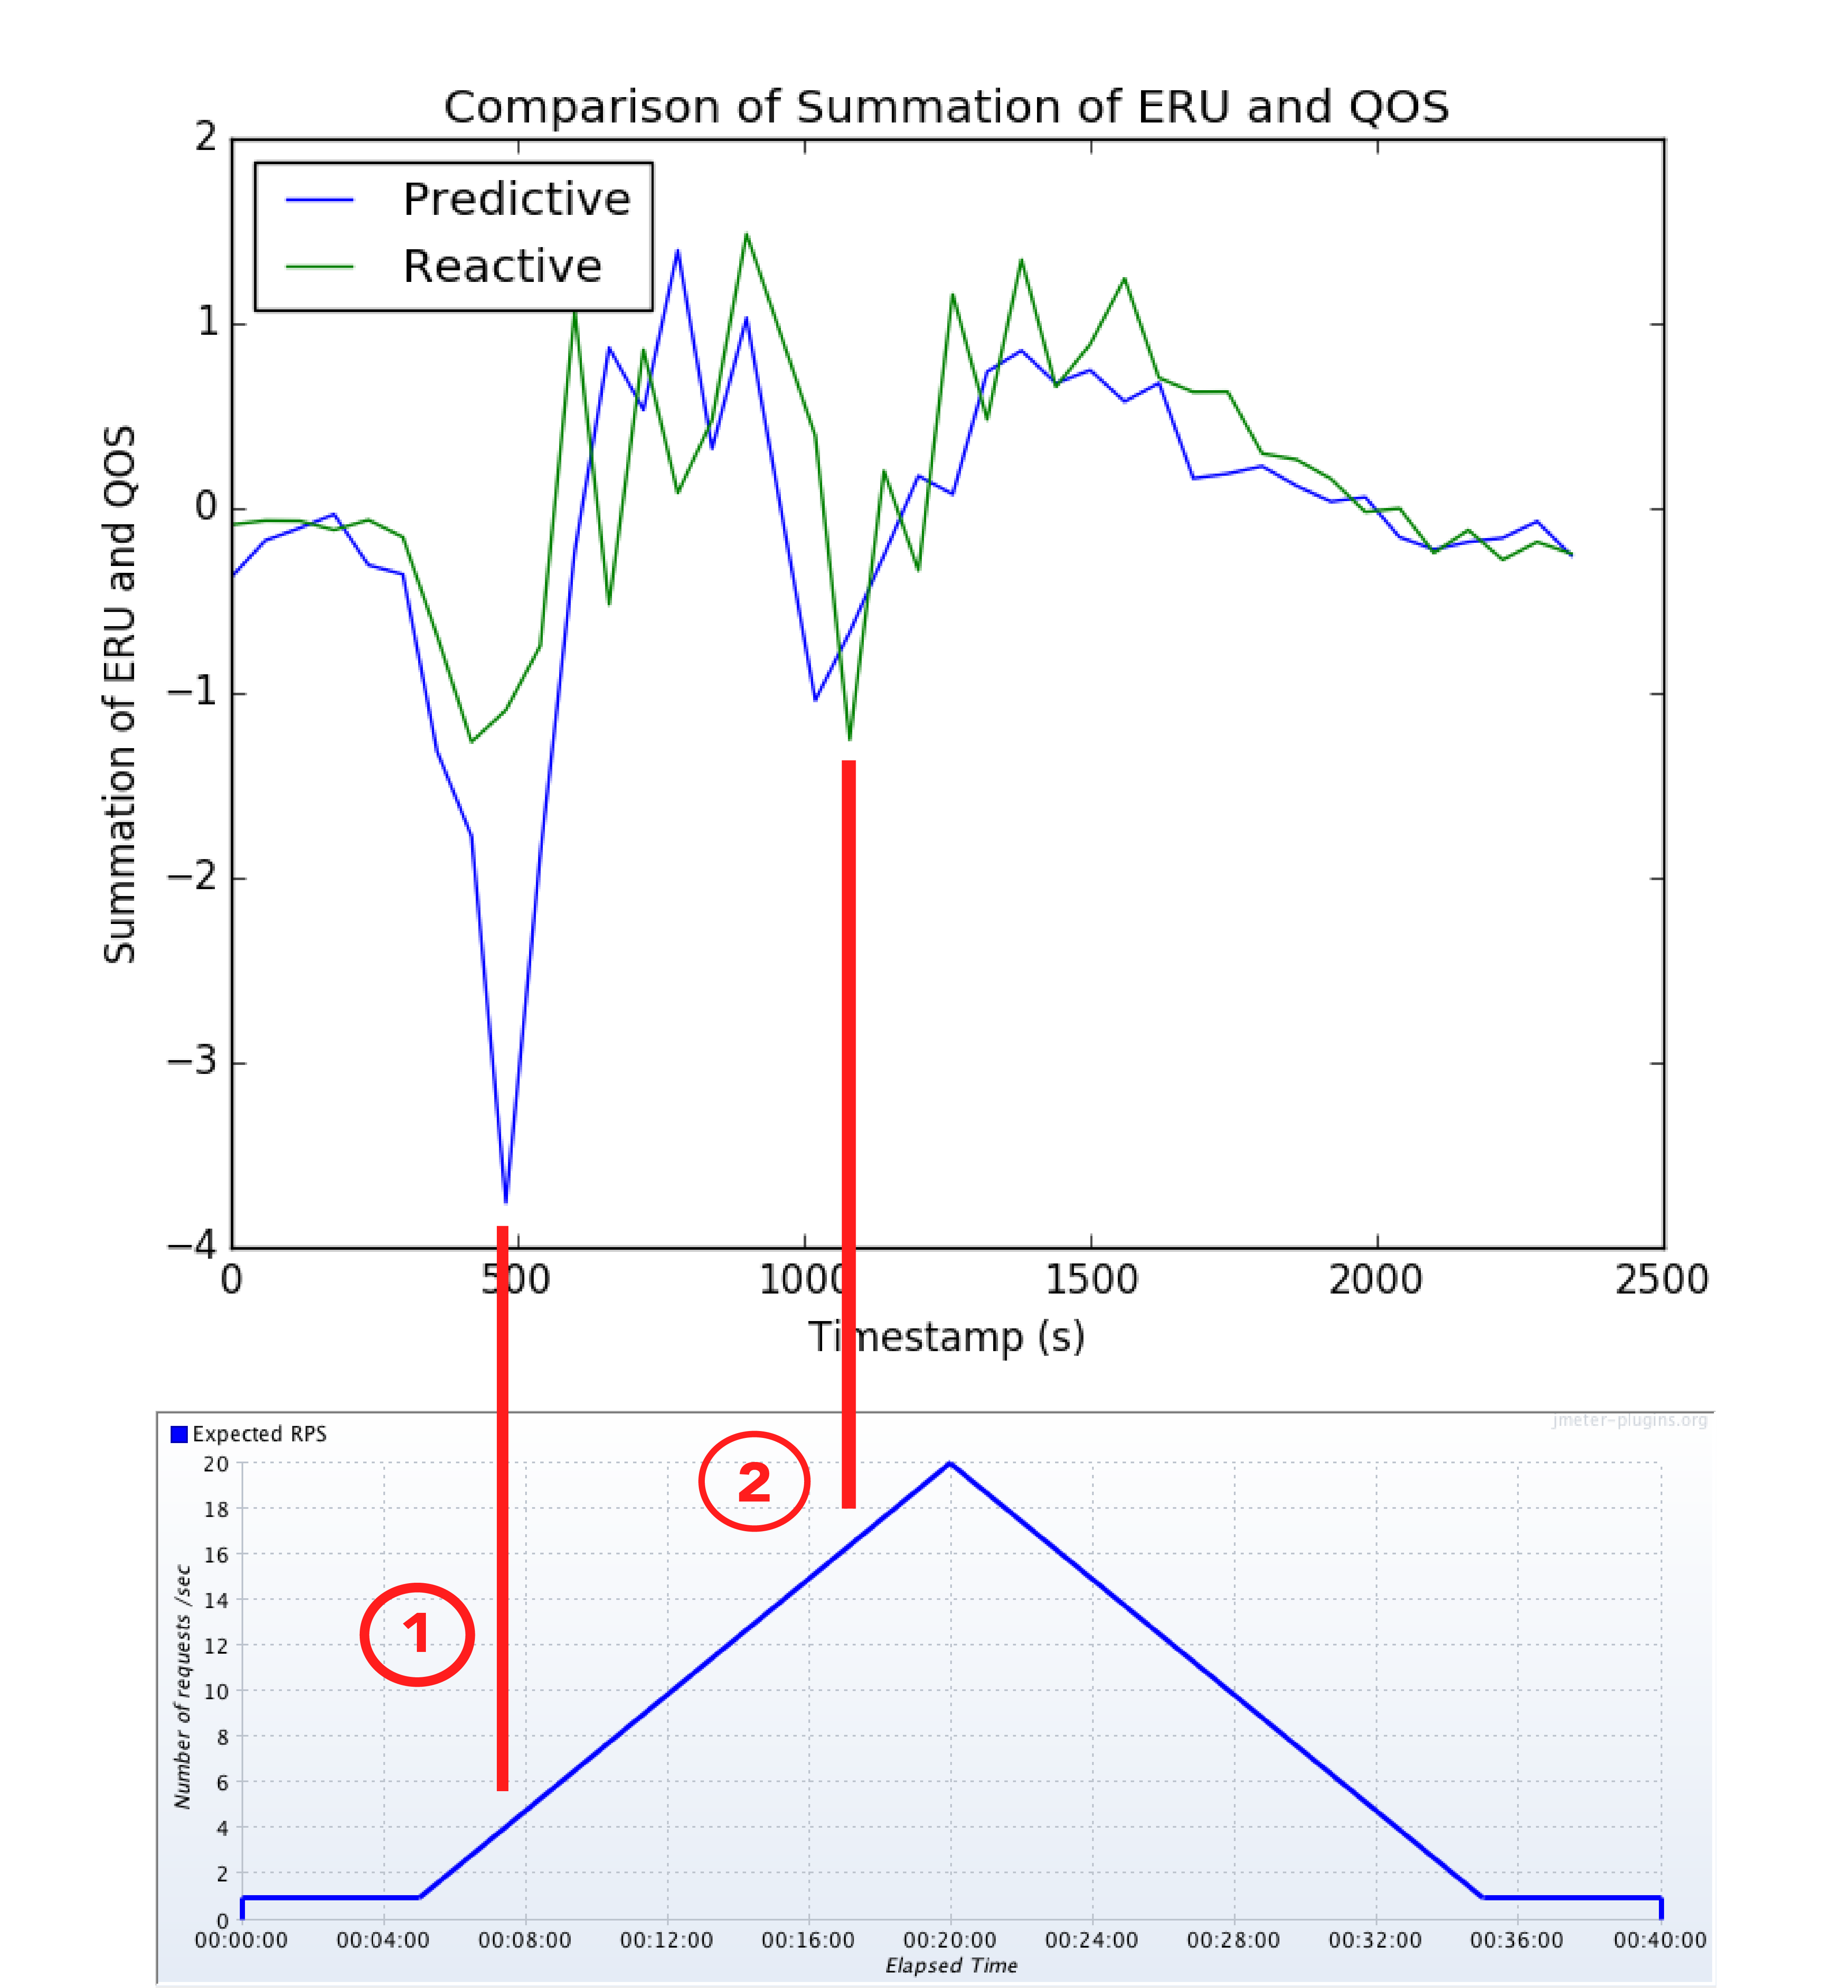
\includegraphics[scale=.70]{increase-decrease-labelled.png}}
  \caption{A comparison of the summation of ERU and QoS for
    predictive and reactive auto-scaling for 135s, increase-decrease.}
  \label{fig:135s-increase-decrease-labelled}
\end{figure}

Figure \ref{fig:135s-increase-decrease-labelled} contains a graph
showing predictive and reactive auto-scaling's different
summations of efficient resource utilization and quality of service over the
course of the \textit{increase-decrease} trial. In contrast to our previous two
traffic patterns, we find that predictive auto-scaling is not particularly
beneficial in this context. Specifically, if we look at the moment labelled
$1$ on Figure \ref{fig:135s-increase-decrease-labelled}, we an instance in which
predictive auto-scaling suffers a severe performance decrease in comparison to
reactive auto-scaling. We trace this decrease again to under-provisioning. In
this scenario, the introductory buffer period has caused our linear prediction
algorithm to underestimate the slope of the line indicating the rise in load. As
such, the reactive auto-scaling algorithm actually has a more aggressive opinion
of the load the application will face. As this aggressive understanding is
confirmed by our actual increase, reactive auto-scaling outperforms predictive
auto-scaling on the \textit{increase-decrease} traffic-pattern. Scenario
$1$ is in contrast to the scenario labelled $2$, in which predictive
auto-scaling performs equally to reactive auto-scaling, because it is no longer
negatively impacted by previous measurements which do not reflect the current
slope.

\begin{table}[htbp]
  \centering
  \caption{Difference in Predictive and Reactive Auto-scaling for 135s,
  increase-decrease.}
  \label{tab:135s-increase-decrease}
\begin{tabular}{l c}\hline\hline
    \multicolumn{1}{c}{\textbf{Measure}} & \textbf{Value} \\ \hline
     p-value & 0.638 \\
     z-score & -.0352 \\
     std\_dev & 0.680 \\
     mean & -0.234
  \end{tabular}
\end{table}

Figure \ref{fig:135s-increase-decrease-labelled} shows that predictive
auto-scaling is actually slightly detrimental on
the \textit{increase-decrease} traffic pattern.
Still, Table \ref{tab:135s-increase-decrease} shows that we are not able to claim
statistical significance with respect to these results, and thus should not be
too confident that prediction has a negative effect. Rather, it appears to
have very little impact in either direction on this traffic pattern.


\subsubsection{135s and flash-crowd}

\begin{figure}[!h]
  \centerline{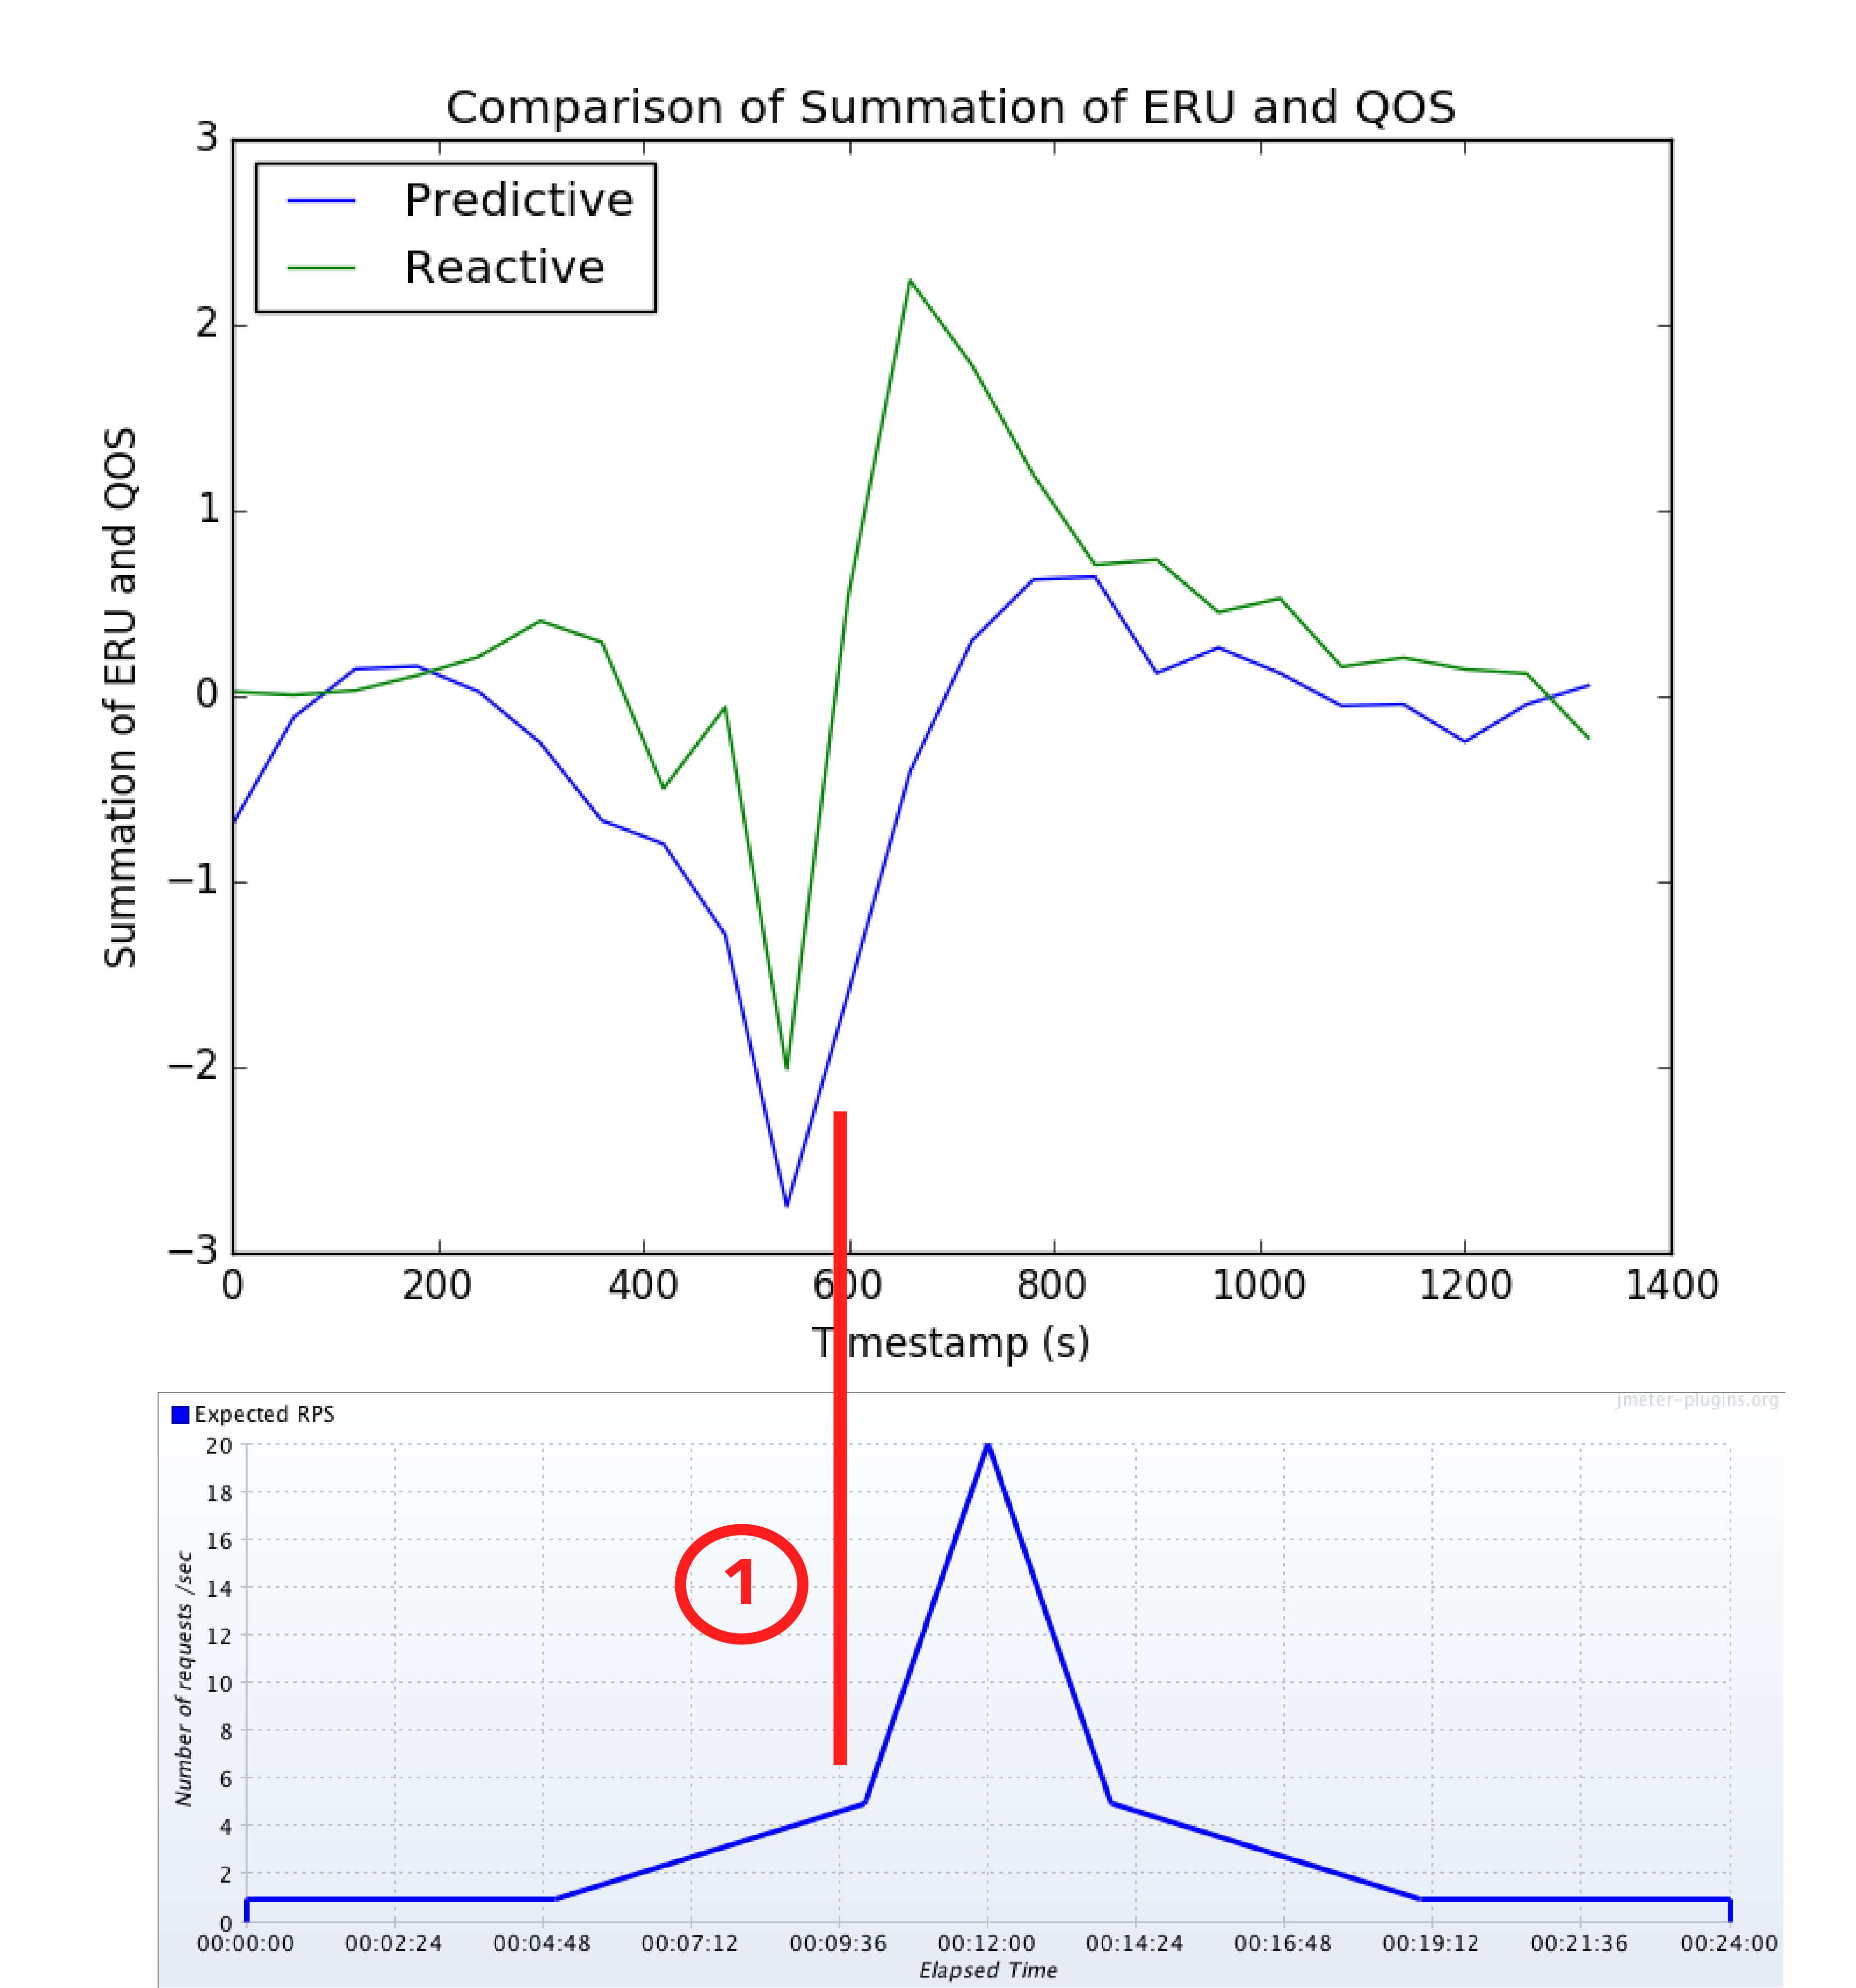
\includegraphics[scale=.70]{flash-crowd-short-labelled.png}}
  \caption{A comparison of the summation of ERU and QoS for
    predictive and reactive auto-scaling for 135s, flash-crowd.}
  \label{fig:135s-flash-crowd-labelled}
\end{figure}

Figure \ref{fig:135s-flash-crowd-labelled} contains a graph
showing predictive and reactive auto-scaling's different
summations of efficient resource utilization and quality of service over the
course of the \textit{flash-crowd} trial. Again,
we find that predictive auto-scaling is not particularly
beneficial in this context. Specifically, if we look at the moment labelled
$1$ on Figure \ref{fig:135s-flash-crowd-labelled}, we see another instance in which
predictive auto-scaling suffers a severe performance decrease because of
under-provisioning. Because this traffic pattern occurs over such a short
interval, the predictive auto-scaling algorithm is unable to fully recognize and
respond to the flash crowd, and is instead hampered by previous measurements
with a significantly lesser slope. Our line-of-best-fit for prediction has too
small a slope, and thus predictive auto-scaling functions worse than reactive
auto-scaling.

\begin{table}[htbp]
  \centering
  \caption{Difference in Predictive and Reactive Auto-scaling for 135s,
  flash-crowd.}
  \label{tab:135s-flash-crowd}
\begin{tabular}{l c}\hline\hline
    \multicolumn{1}{c}{\textbf{Measure}} & \textbf{Value} \\ \hline
     p-value & 0.802 \\
     z-score & -.850 \\
     std\_dev & 0.695 \\
     mean & -0.591
  \end{tabular}
\end{table}

Figure \ref{fig:135s-flash-crowd-labelled} shows that predictive
auto-scaling is fairly detrimental on the \textit{flash-crowd} traffic pattern.
Given Table \ref{tab:135s-flash-crowd}, we are still not able to claim
statistical significance with respect to these results, but we should be fairly
confident that this current iteration of predictive auto-scaling is not an advisable addition
when expecting flash crowds.



\subsection{Scenarios}

Given the evaluation of a typical application benefiting from horizontal
auto-scaling on two distinct test patterns, we can comment on the general
scenarios in which predictive auto-scaling is effective and beneficial, and the
situations in which reactive auto-scaling is either less effective or
detrimental.

To begin, we consider when predictive auto-scaling is less
effective. Predictive auto-scaling offers little distinction from reactive
auto-scaling when the pod initialization time approaches 0s. Thus, predictive
auto-scaling is not particularly interesting for containerized web server
applications. This lack of difference is particularly noticeable given the
multi-minute threshold Kubernetes imposes between when auto-scalings can occur.
Our decision to not even evaluate a 5s pod initialization time reflected our
understanding of the lack of utility for predictive auto-scaling for web servers
that start particularly quickly.

Predictive auto-scaling has a greater positive and negative impact
with a longer pod initialization time, as we saw when auto-scaling on an
application simulating downloading shard data. From our graphs, we could see
repeatable performance differences, and scenarios in which predictive
auto-scaling offered the most benefits and scenarios in which reactive
auto-scaling offered the most benefits. Specifically, predictive auto-scaling
allows us to respond to quickly to increases in load, ensuring that we
substantially react to initial spikes. While such behavior is beneficial in the
immediate aftermath of increased load, it can raise challenges if an even
greater scaling would otherwise be performed at a time within the
threshold Kubernetes imposes in
which scaling cannot occur. Particularly if predictive auto-scaling
underestimated the initial amount to scale, or only created a small replica
number of pods, scaling too early can lead to
performance decreases during the threshold period. Reactive auto-scaling avoids
these performance decreases by performing its scaling actions during period of
peak load, and thus creating greater replica pods. In short, predictive
auto-scaling offers a trade off between quickly and immediately responding to
increased load, while taking the risk that even greater increases during the
threshold time while go unaddressed until the threshold period ends.

With an eye towards the real-world, there are a variety of scenarios in
predictive auto-scaling would be particularly useful. Specifically, the ability
to ensure we respond aggressively to an initial burst in traffic corresponds
nicely with notification services which will notify users and then achieve a
very steep, quick increase in users, before an equally steep decline. If this
burst occurs within the span of the threshold in which auto-scaling is
prevented, there will be no penalty to predictive auto-scalings aggressive
scaling. Furthermore, we can examine other scenarios in which we would rather
have high performance at the beginning of a heavy load period than the end. For
example, if we have a peer to peer system established in which all nodes in the
system originally query a single node, until they themselves have the
information and can be queriable, we would prefer a predictive auto-scaling
implementation. Predictive auto-scaling should sufficiently handle the initial
burst, and if there are any performance degradations during the threshold
period, they will be in part diminished by the previous successful queries of
the first node ensuring other nodes have the data and can thus serve as
additional replicas. This performance is in comparison to reactive auto-scaling,
which may not be able to handle the additional burst, and thus the system would
crash as no nodes would have been able to get the shared data. There are likely
a variety of additional operations and systems matching this general theme in
which predictive auto-scaling is particularly useful.



\section{Implications}

\input{chapters/evaluation/implications}

\section{Summary}

Overall, there are a number of lessons to be learned in this section. In
summation, we discussed the variety of methods for performing resource intensive
computational tasks, before focusing on cluster computing. We examined a variety
of popular cluster managers, before focusing on Kubernetes. Finally, we examined
a variety of methods of auto-scaling applications running on cluster managers,
before focusing on model predictive control. The remainder of this thesis will
seeks to show the effectiveness of model predictive control in modifying the
current implementation of auto-scaling in Kubernetes, such that we will improve
both quality of service and efficient resource utilization.


